\documentclass[../main.tex]{subfiles}

\begin{document}

    \subsection{Jakość oprogramowania}
    Jakości jest pojęciem \textbf{niejednoznacznym} i \textbf{wielowymiarowym}.

    Różne spojrzenia wg Garvina:
    \begin{itemize}
        \item jakość oparta na \textbf{produkcie} (np. charakterystyki jakościowe)
        \item jakość oparta na \textbf{użytkowniku} (funkcjonalność, fitness for use)
        \item jakość oparta na \textbf{wytwarzaniu} (jakość „techniczna” procesu)
        \item jakość oparta na \textbf{wartości} (czas vs. wysiłek vs. koszt)
        \item jakość \textbf{transcendentna} (nieoperacyjna, trudno mierzalna, np. „grywalność” gry komputerowej)
    \end{itemize}


    \subsubsection{Model jakości ISO 9126}
    \begin{figure}[H]
        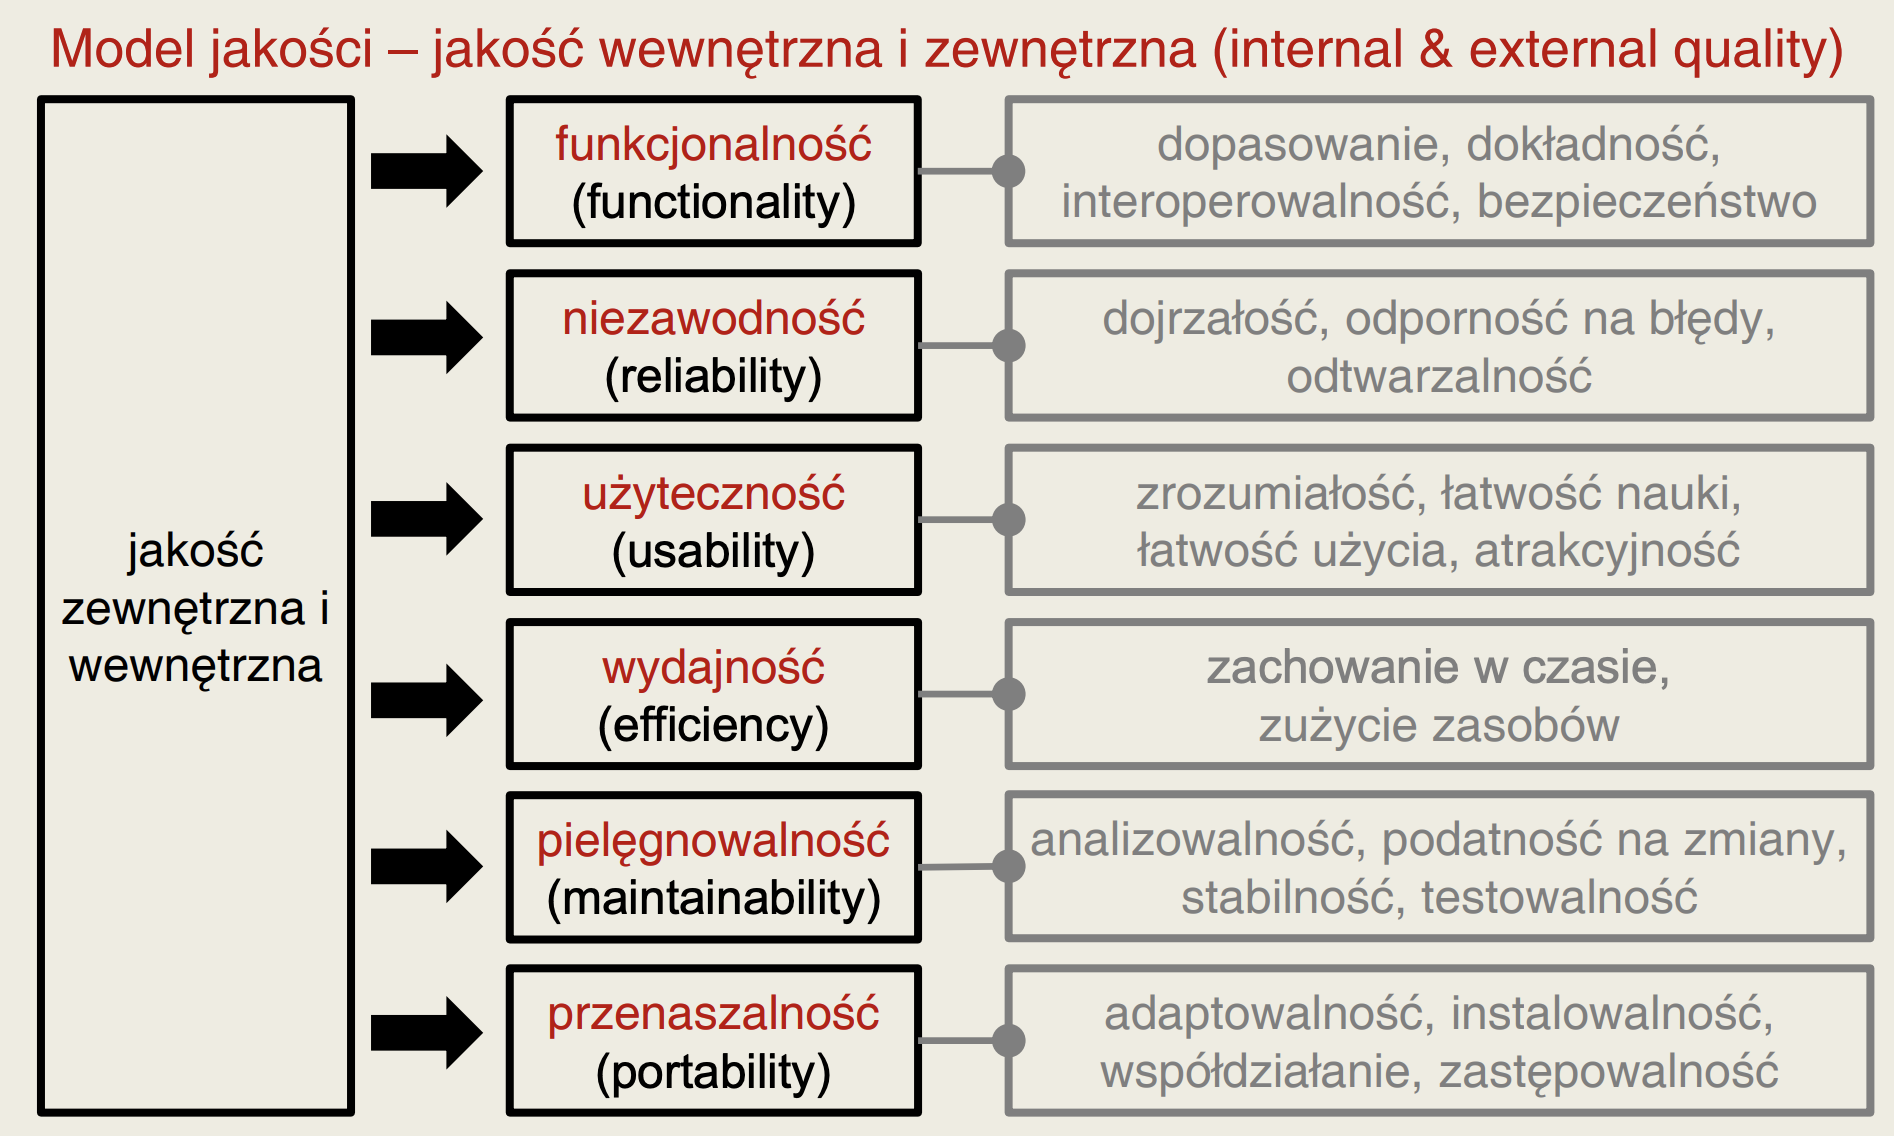
\includegraphics[width=\linewidth]{ISO9126_1.png}
    \end{figure}

    \begin{figure}[H]
        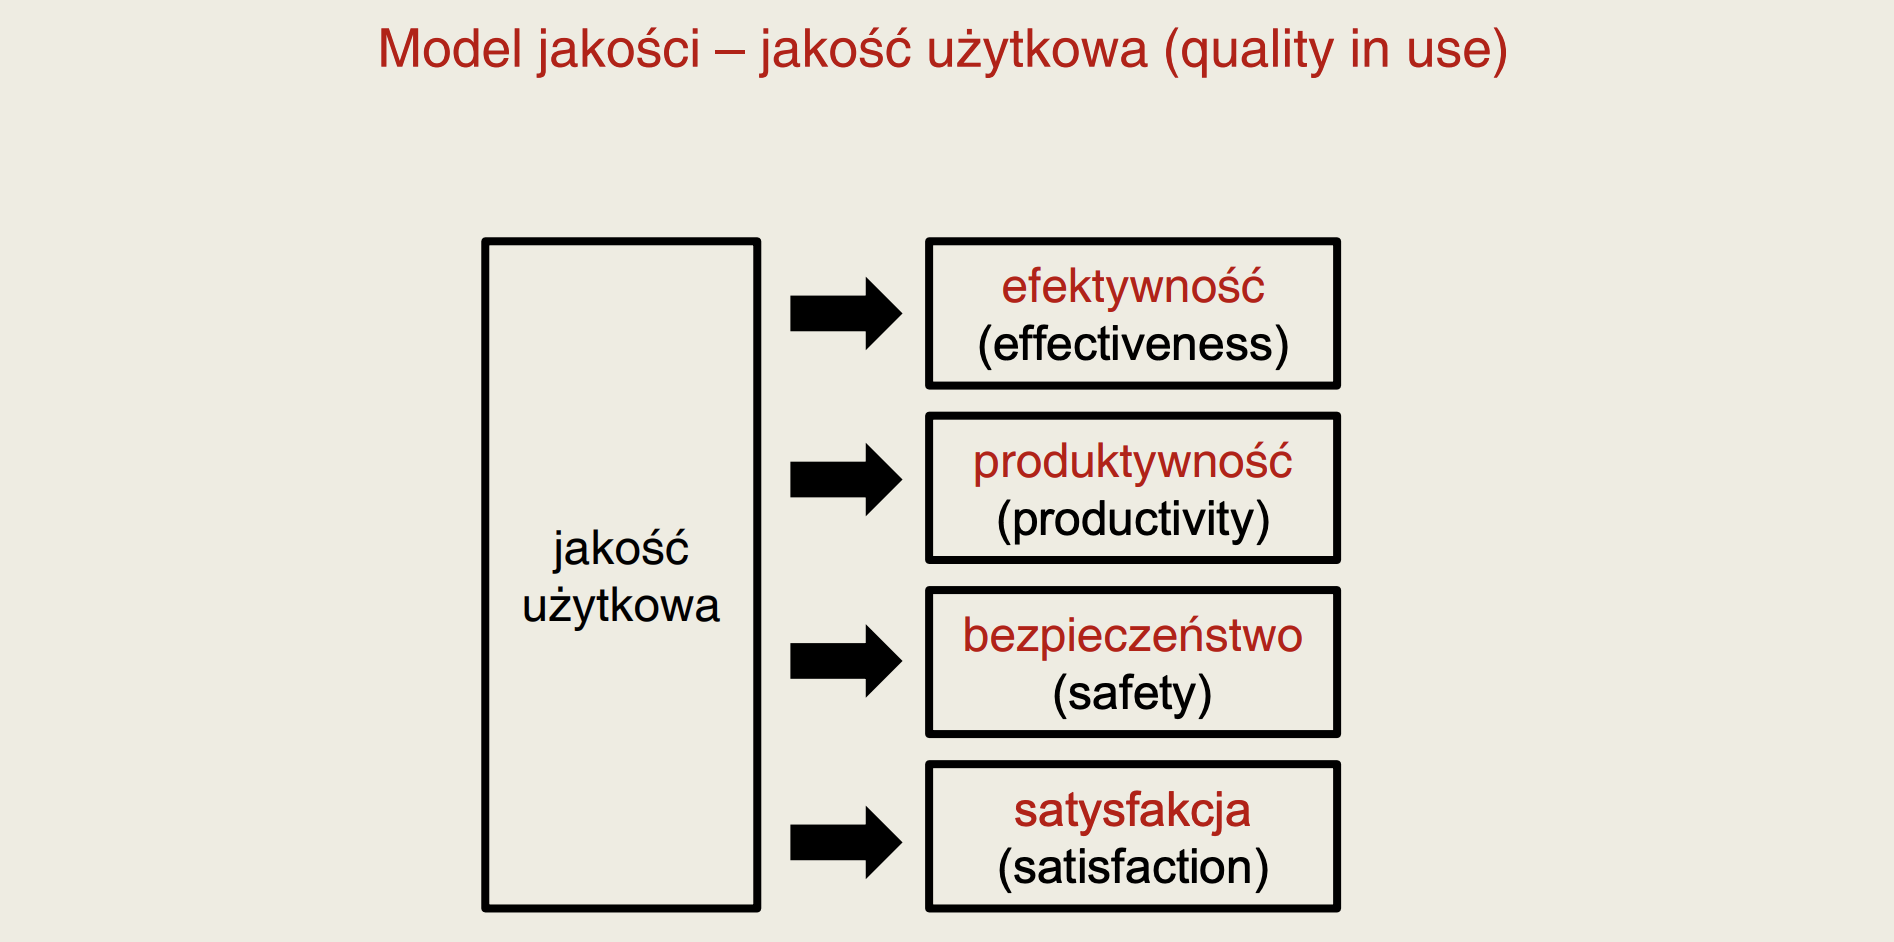
\includegraphics[width=\linewidth]{ISO9126_2.png}
    \end{figure}

    \subsubsection{Model jakości ISO/IEEE 25000}
    Nowa rodzina norm, zastępująca starą normę 9126.


    Jakość produktu (system/software product quality):
    \begin{itemize}
        \item funkcjonalna przydatność
        \item wydajność w działaniu
        \item zgodność
        \item użyteczność
        \item niezawodność
        \item bezpieczeństwo
        \item pielęgnowalność
        \item przenaszalność
    \end{itemize}

    Jakość użytkowa (quality in use)
    \begin{itemize}
        \item efektywność
        \item wydajność
        \item satysfakcja
        \item wolność od ryzyka
        \item kontekst użycia
    \end{itemize}



    \subsubsection{Niezawodność}

    \textbf{Niezawodność} - zdolność oprogramowania do bezbłędnego działania przez określony czas lub przez określoną
    liczbę operacji.

    Testy niezawodności wykorzystują \textbf{profile operacyjne}.

    Cechy niezawodności:
    \begin{itemize}
        \item dojrzałość (zdolność do bezawaryjnego działania przy występowaniu usterek)
        \item tolerancja na błędy (np. obsługa wyjątków)
        \item odtwarzalność (zdolność działania po awarii)
    \end{itemize}

    \begin{figure}[H]
        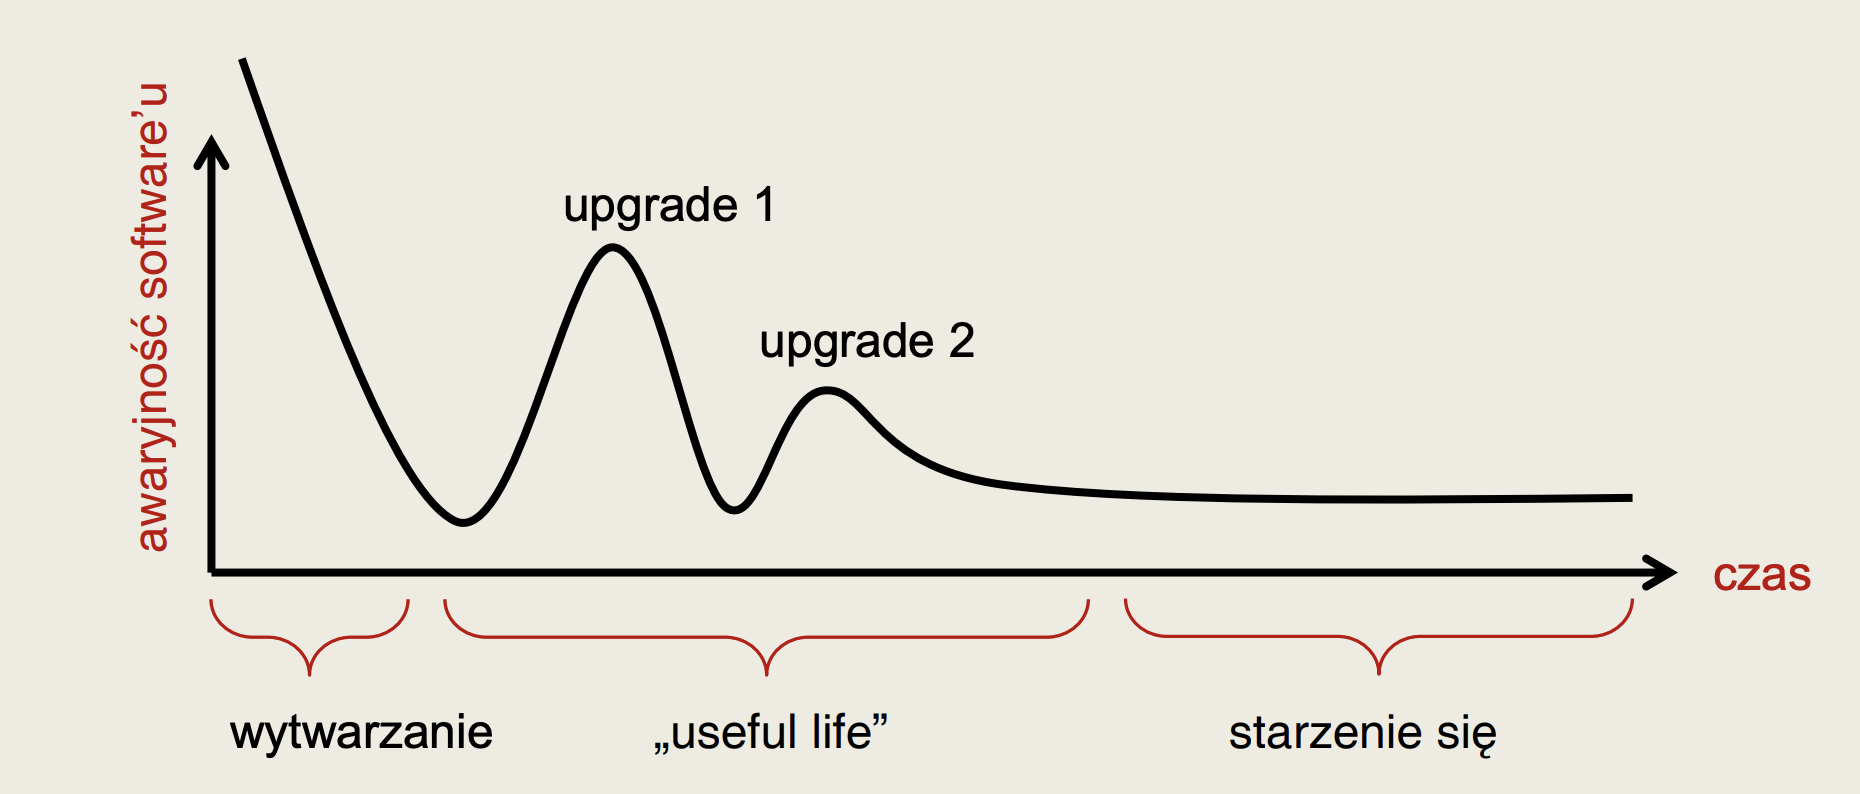
\includegraphics[width=\linewidth]{niezawodnosc.png}
    \end{figure}

    \begin{figure}[H]
        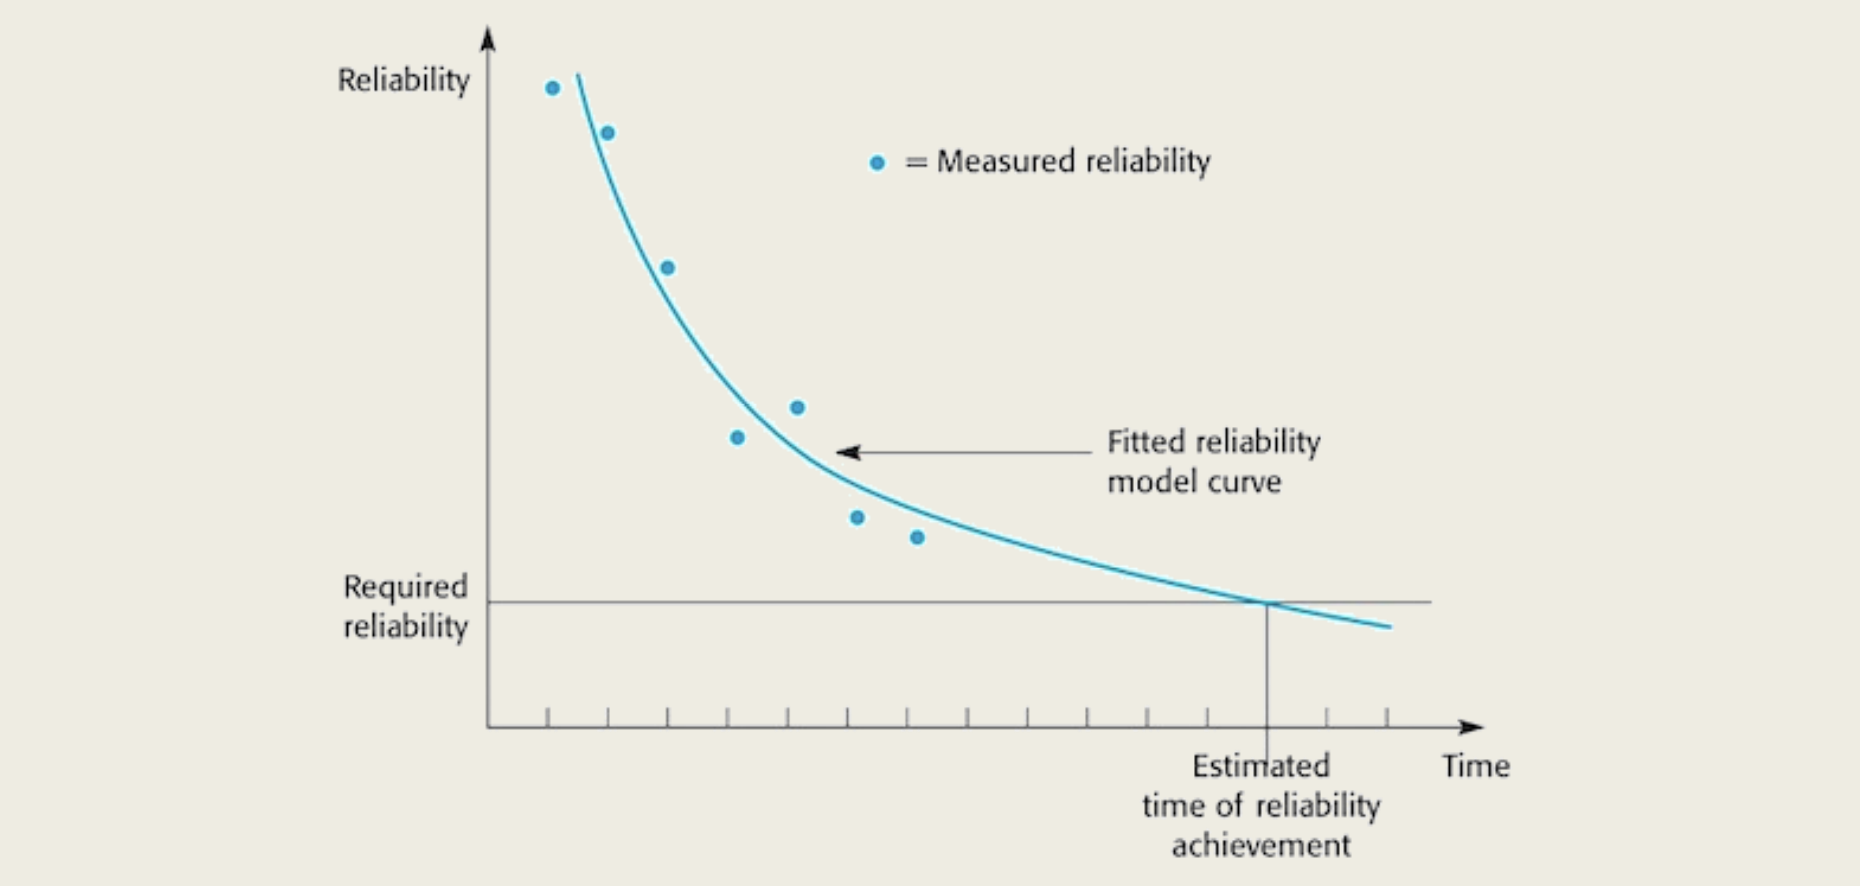
\includegraphics[width=\linewidth]{predniez.png}
    \end{figure}


    \textbf{Metryki}
    \begin{figure}[H]
        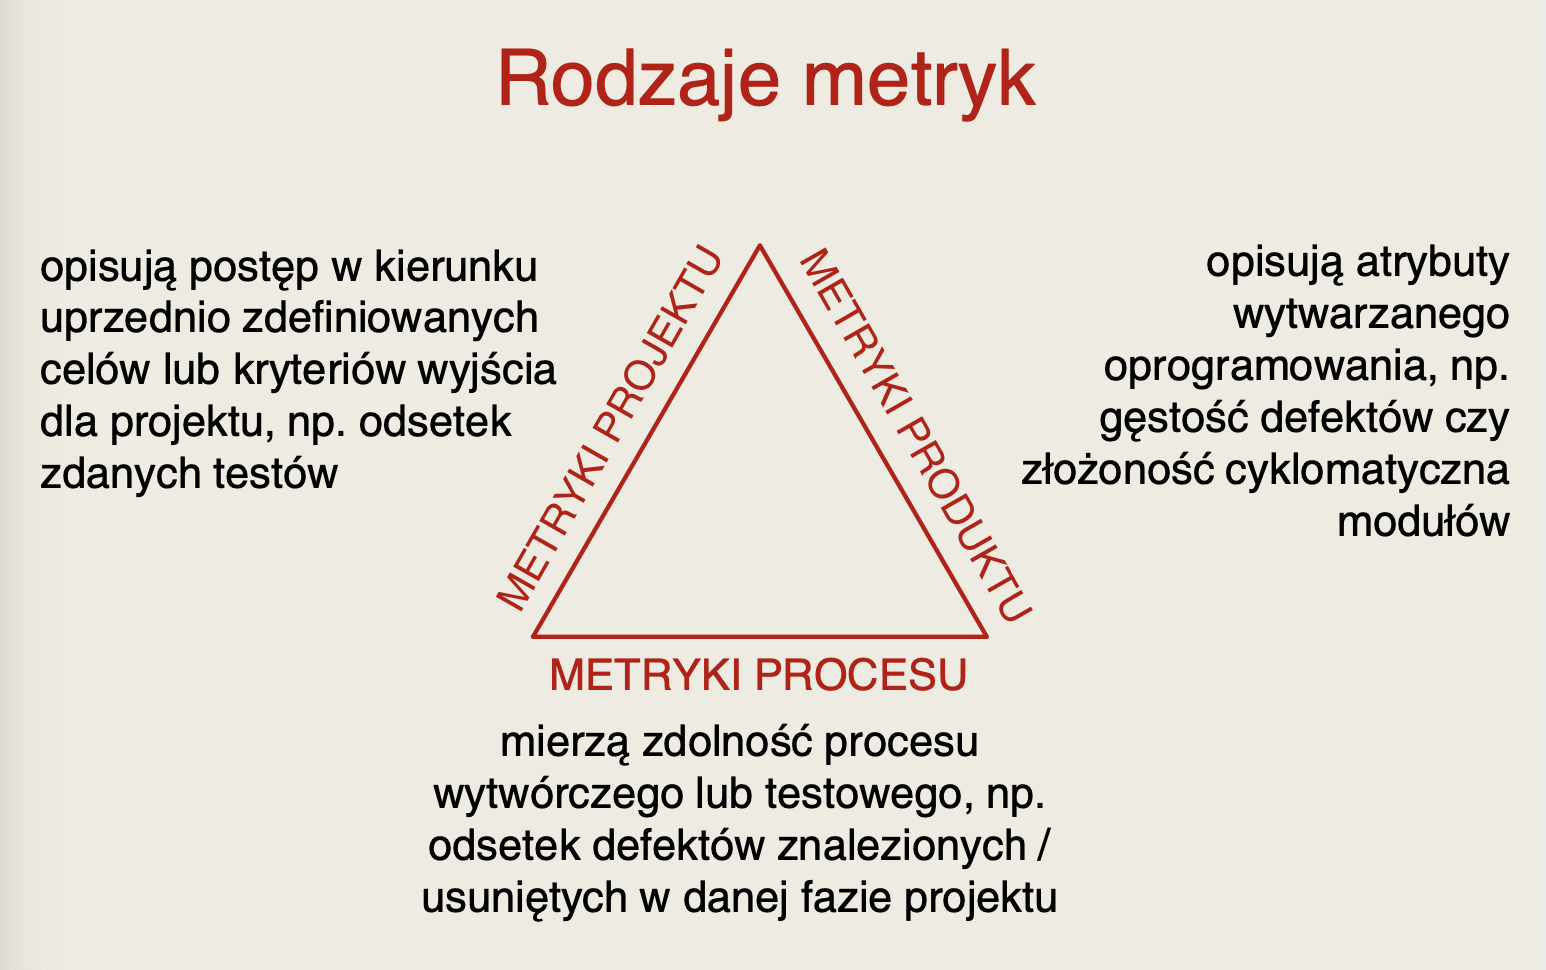
\includegraphics[width=\linewidth]{metryki.png}
    \end{figure}

    $MTTF$ = Mean Time To Failure (średni czas do awarii)
    $MTTR$ = Mean Time To Repair (średni czas do naprawy)
    $MTBF$ = Mean Time Between Failures (średni czas między awariami)

    \begin{align*}
        MTTF = \frac{\sum_{i=1}^{N} OK_i}{N}
    \end{align*}

    \begin{align*}
        MTTR = \frac{\sum_{i=1}^{N} R_i}{N}
    \end{align*}

    \begin{align*}
        MTBF = MTTF + MTTR
    \end{align*}

    Wraz ze wzrostem dojrzałości oprogramowania MTTF wzrasta


    \subsubsection{Bezpieczeństwo}
    \begin{itemize}
        \item Bezpieczeństwo to zbiór atrybutów oprogramowania umożliwiający ochronę przed nieautoryzowanym
        dostępem do programu i danych
        \item Często zagrożenia bezpieczeństwa są ukryte, niejawne i niewidoczne
        \item Błędy bezpieczeństwa często nie mają widocznych symptomów (nawet po włamaniu)
        \item Profesjonalne testy bezpieczeństwa zwykle wykonywane przez zewnętrzne, wyspecjalizowane w tym obszarze firmy
    \end{itemize}

    Przykłady:
    \begin{itemize}
        \item piractwo (nieautoryzowany dostęp do danych) -SQL injection, hasła, pliki tymczasowe, fizyczna lokalizacja serwera
        \item przepełnienie bufora
        \item DoS (Denial of Service)
        \item przechwycenie transferu danych
        \item łamanie zabezpieczeń (kryptologia)
        \item bomby logiczne, wirusy, robaki
        \item social engineering – pretexting, phishing, itp
    \end{itemize}

    \textbf{OWASP}, Open Web Application Security Project - obszerna baza zasobów dot. bezpieczeństwa webowego, np.:
    \begin{itemize}
        \item baza ataków
        \item baza książek i innych materiałów o bezpieczeństwie
        \item portal społecznościowy
        \item projekty związane z bezpieczeństwem
        \item dokumentacja, modele
        \begin{itemize}
            \item SAMM = Software Assurance Maturity Model
            \item model pozwalający organizacji zdefiniować i wdrożyć strategię dla zapewnienia bezpieczeństwa,
            dopasowaną do określonych ryzyk
        \end{itemize}
    \end{itemize}

    \subsubsection{Użyteczność}
    \begin{itemize}
        \item Użyteczność to zdolność systemu do bycia zrozumiałym, łatwym do nauczenia i użycia oraz atrakcyjnym dla
        użytkownika
        \item Testowanie skupia się na użytkownikach i ich działaniu.
        \item Efekty testowania obserwowane na prawdziwych, końcowych użytkownikach, a nie testerach
        \item Testowanie użyteczności wymaga wiedzy psychologicznej, socjologicznej, z zakresu ergonomii, standardów dot.
        dostępności
    \end{itemize}


    \textbf{Podcharakterystyki}
    \begin{itemize}
        \item \textbf{Zrozumiałość} - jak łatwo zrozumieć co program robi i dlaczego mielibyśmy go używać?
        \item \textbf{Łatwość nauki} - łatwość zrozumienia jak program działa
        \item \textbf{Łatwość obsługi} - czy obsługa programu jest intuicyjna?
        \item \textbf{Atrakcyjność} - czy użytkownik chętnie używa programu?
    \end{itemize}

    \textbf{Metryki}\\
    Testowanie użyteczności jest ukierunkowane na pomiar:
    \begin{itemize}
        \item \textbf{efektywności}
        \begin{itemize}
            \item np. stopień osiągnięcia przez użytkownika celów, z
            określoną dokładnością i zupełnością
        \end{itemize}
        \item \textbf{wydajności}
        \begin{itemize}
            \item ilość zasobów zużytych do osiągnięcia celów, np. czas,
            liczba kliknięć itp.
        \end{itemize}
        \item \textbf{satysfakcji} klienta z użytkowania produktu
    \end{itemize}

    \textbf{Testowanie użyteczności}
    \begin{itemize}
        \item \textbf{Proces}
        \begin{itemize}
            \item \textbf{Formatywne} testowanie użyteczności - przeprowadzane iteracyjnie w
            kolejnych fazach projektowania i prototypowania, aby ukierunkować
            (lub „uformować”) projekt poprzez identyfikację defektów użyteczności
            \item \textbf{Całościowe} testowanie użyteczności - przeprowadzane po implementacji
            aby mierzyć użyteczność oraz identyfikować problemy z systemem
            lub komponentem traktowanym całościowo
        \end{itemize}

        \item \textbf{Rodzaje}
        \begin{itemize}
            \item \textbf{Formalne} testowanie użyteczności - często wymaga uprzedniego przygotowania rzeczywistych
            lub reprezentatywnych użytkowników (dostarczenie scenariuszy zadań, instrukcji)
            \item \textbf{Nieformalne} testowanie użyteczności - pozwala użytkownikowi eksperymentować z
            oprogramowaniem, aby obserwatorzy ocenili jak trudna dla użytkownika jest praca z systemem
        \end{itemize}

        \item Walidacja powinna być przeprowadzona w warunkach tak bliskich rzeczywistym warunkom użytkowania
        oprogramowania, jak to tylko możliwe, np. w \textbf{laboratorium użyteczności}.\\

        \item \textbf{Wytyczne} (guidelines) są stosowane aby uzyskać spójne podejście do wykrywania i raportowania defektów
        użyteczności na wszystkich etapach cyklu życia. Powinny zawierać rzeczy takie jak:
        \begin{itemize}
            \item dostępność instrukcji,
            \item klarowność komunikatów,
            \item \# kliknięć do ukończenia zadania,
            \item komunikaty o błędach,
            \item układ elementów na ekranie,
            \item użycie kolorów, dźwięków itp.
        \end{itemize}

        \item \textbf{Specyfikacja} testów użyteczności
        \begin{itemize}
            \item \textbf{Inspekcja, ewaluacja, lub przegląd}
            \begin{itemize}
                \item \textbf{Wymagania i specyfikacja}.
                \item Heurystyczna ocena projektu GUI
                \item Efektywniejsze, gdy UI jest bardziej widoczny, np. są screenshoty
            \end{itemize}

            \item \textbf{Dynamiczna interakcja z prototypami}
            \begin{itemize}
                \item Praca z \textbf{prototypami} i pomoc deweloperom w ich rozwijaniu
                \item Prototypy mogą być przez uzyskanie realistycznego oglądu użytkowników
            \end{itemize}

            \item \textbf{Weryfikacja i walidacja bieżącej implementacji}
            \begin{itemize}
                \item Weryfikacja przy pomocy \textbf{przypadków testowych}, czy oprogramowanie ma cechy użyteczności
                zdefiniowane w wymaganiach
                \item Walidacja przez scenariusze testowe(np. łatwość nauki)
            \end{itemize}

            \item \textbf{Ankiety i kwestionariusze}
            \begin{itemize}
                \item Zbieranie \textbf{obserwacji} i \textbf{informacji zwrotnej} dotyczącej zachowania użytkowników
                \item \textbf{SUMI} (Software Usability Measurement Inventory), \textbf{WAMMI} (Website Analysis and MeasureMent Inventory)
                – standaryzowane benchmarki
            \end{itemize}
        \end{itemize}
    \end{itemize}

    \subsubsection{Wydajność}
    \begin{itemize}
        \item Zdolność oprogramowania do zapewnienia odpowiedniej efektywności w działaniu, relatywnie do
        ilości zużytych zasobów
        \item Systemy o znaczeniu krytycznym muszą dostarczać swoje funkcje w ściśle określonym czasie
        \item Dla systemów czasu rzeczywistego (i innych) ważne jest zużycie zasobów
    \end{itemize}

    \textbf{Błędy wydajności} powodują:
    \begin{itemize}
        \item wolny czas odpowiedzi
        \item nieadekwatną przepustowość
        \item problemy z niezawodnością (obciążenie)
        \item nadmierne wymagania co do zasobów
    \end{itemize}

    Najczęstsza przyczyna błędów wydajności: błędy projektowe (a więc trudne do usunięcia w późniejszych fazach testów).

    Testowanie wydajności powinno być przeprowadzane na każdym etapie cyklu życia – zwłaszcza w fazie projektu i kodowania.

    \textbf{Rodzaje testów} wydajności:
    \begin{itemize}
        \item testowanie \textbf{obciążenia} (load testing)
        \item testowanie \textbf{warunków skrajnych} (stress testing)
        \item testowanie \textbf{skalowalności} (scalability testing)
        \item testowanie \textbf{wykorzystania zasobów} (resource utilization testing)
        \item testowanie \textbf{wytrzymałościowe} (endurance testing)
        \item testowanie \textbf{skokowe} (spike testing)
        \item testowanie \textbf{niezawodności} (reliability testing)
        \item testowanie \textbf{z aktywnym tłem} (background testing)
        \item testowanie \textbf{punktu krytycznego} (tip-over testing)
    \end{itemize}

    Przykładowe \textbf{metryki} dla wydajności:
    \begin{itemize}
        \item \% wykorzystania procesora w kluczowym czasie
        \item dostępna pamięć (RAM, wirtualna)
        \item top N aktywnych procesów
        \item liczba przełączeń kontekstów na sekundę
        \item długość kolejek (procesor, dysk) w danym czasie
        \item zużycie i wysycenie pamięci dyskowej
        \item błędy sieci
        \item czas podróży pakietu
        \item czas prezentacji danych klientowi
    \end{itemize}

    \begin{figure}[H]
        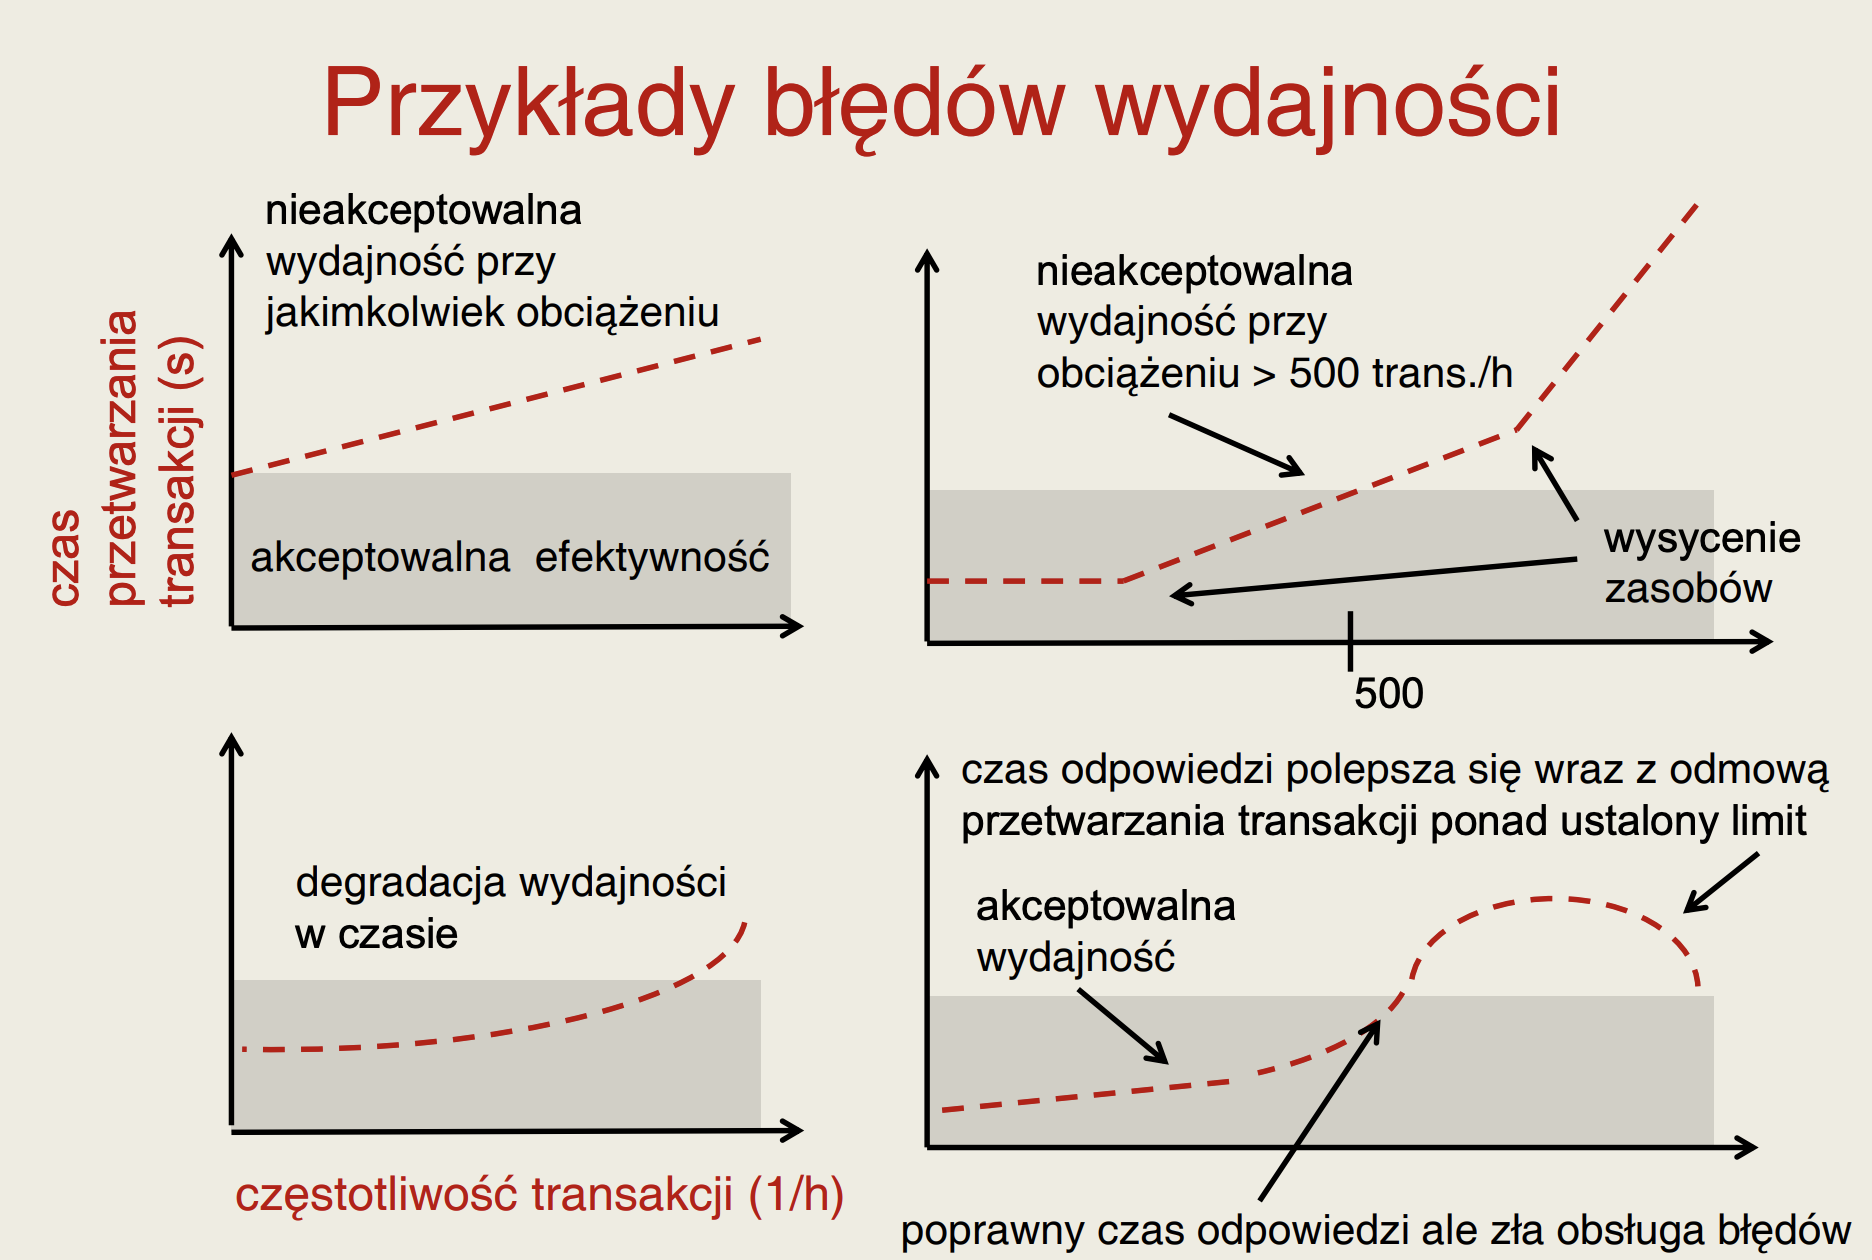
\includegraphics[width=\linewidth]{bledywyd.png}
    \end{figure}

    \subsubsection{Pielęgnowalność}
    \begin{itemize}
        \item Pielęgnowalność to łatwość modyfikowania oprogramowania w celu naprawy defektów, dostosowania do nowych
        wymagań, ułatwienia przyszłego utrzymywania lub dostosowania do zmian zachodzących w jego środowisku
        \item Oprogramowanie się nie zużywa, ale staje się przestarzałe
        \item Zatem będą pojawiać się:
        \begin{itemize}
            \item nowe funkcjonalności
            \item patche
            \item aktualizacje oprogramowania
            \item nowe środowiska
        \end{itemize}
    \end{itemize}

    \textbf{Testowanie pielęgnowalności}\\
    \begin{itemize}
        \item Zwykle nie przy pomocy skryptów testowych
        \item Większość defektów związanych z pielęgnowalnością jest niewidoczna dla testowania dynamicznego
        \item Defekty te są bowiem powodowane m.in.:
        \begin{itemize}
            \item trudnym do zrozumienia kodem
            \item zależnościami środowiskowymi
            \item ukrytymi informacjami i stanami
            \item złą architekturą
            \item użyciem złej technologii
        \end{itemize}
        \item Wniosek: najlepiej sprawdzają się techniki statyczne
    \end{itemize}

    \textbf{Podcharakterystyki} pielęgnowalności i \textbf{problemy} z nimi związane:
    \begin{itemize}
        \item \textbf{Analizowalność} - łatwość diagnozowania problemów
        \begin{itemize}
            \item spaghetti code
            \item brak dobrej dokumentacji
            \item brak lub złe standardy/zalenia
            \item abstrakcja kodu
        \end{itemize}

        \item \textbf{Modyfikowalność} - zdolność do wprowadzania zmian
        \begin{itemize}
            \item związanie (coupling)
            \item brak kohezji
            \item zły styl kodowania
            \item kiepska dokumentacja
        \end{itemize}

        \item \textbf{Stabilność} - zdolność do unikania niespodziewanych efektów na skutek zmian
        \begin{itemize}
            \item związanie
            \item brak kohezji
            \item jakośc wymagań
        \end{itemize}

        \item \textbf{Testowalność} - łatwość walidacji po wprowadzonej zmianie
        \begin{itemize}
            \item brak lub zła dokumentacja
            \item brak komentarzy w kodzie
            \item antywzorce projektowe
            \item zła konwencja nazewnictwa
            \item brak instrumentacji kodu
        \end{itemize}
    \end{itemize}

    \subsubsection{Przenaszalność}
    \begin{itemize}
        \item Przenaszalność to \textbf{łatwość}, z jaką oprogramowanie może być przeniesione z jednego środowiska do innego .
        \item Najczęstsze przyczyny problemów z przenaszalnością:
        \begin{itemize}
            \item zależności środowiskowe
            \item zajmowanie zasobów
            \item niestandardowe interakcje systemu operacyjnego
        \end{itemize}
        \item \textbf{Podcharakterystyki} przenaszalności:
        \begin{itemize}
            \item \textbf{Adaptowalność} – zdolność do adaptacji w innym środowisku bez
            podejmowania akcji innych niż przewidziane w tym celu – nie zawsze dobre; nie zawsze tanie i proste (Java)
            \item \textbf{Zastępowalność} – możliwość do bycia zastąpionym przez inny
            produkt do tego samego celu w tym samym środowisku – np. DLL, COM, DCOM, COTS…
            \item \textbf{Instalowalność} – możliwość bycia zainstalowanym w danym środowisku
            – zależności, błędy, niemożność przerwania…
            \item \textbf{Koegzystencja} – zdolność do współistnienia z innym, niezależnym oprogramowaniem dzielącym środowisko
            – np. „przywłaszczenie” standardowego skrótu klawiszowego lub kombinacji dla znaków specjalnych przez inny program
        \end{itemize}
    \end{itemize}
\end{document}